\documentclass[english]{sareport}
% use the option peerreview for creating an anonymized version of your report
% E.g., \documentclass[english,peerreview]{sareport}

\usepackage[colorlinks, linkcolor=black, citecolor=black, urlcolor=black]{hyperref}
\usepackage[normalem]{ulem}

\usepackage{graphicx}
\usepackage{rotating}
\usepackage{enumitem}
\setlist{noitemsep} % \setlist{nosep}

\casename{Shared Internet Of Things Infrastructure Platform}
\phasenumber{2a}
\phasename{ADD Application}

% Set all authors, if your group counts 2, set third author empty \authorthree{}
% Set the groupname as well
\authorone{Monika Filipcikova (r0683254)}
\authortwo{Armin Halilovic(r0679689)}
\authorthree{}
\groupname{Filipcikova-Halilovic}
\academicyear{2016--2017}

\begin{document}
\maketitle

\tableofcontents

\chapter{Attribute-driven design documentation}\label{sec:add}
\section{Decomposition 1: SIoTIP System (Av3, UC14, UC15, UC18)}

\subsection{Module to decompose}
    In this run we decompose the \texttt{SIoTIP System}.


\subsection{Selected architectural drivers}
    The non-functional drivers for this decomposition are:
    \begin{itemize}
    	\item \emph{Av3}: Pluggable device or mote failure
    \end{itemize}

    \noindent The related functional drivers are:
    \begin{itemize}
    	\item \emph{UC14}: Send heartbeat (Av3) \\
              This use case checks whether or not motes and pluggable devices
              are still operational.
    	\item \emph{UC15}: Send notification (Av3) \\
              This use case sends a notification to a registered user.
    	\item \emph{UC18}: Check and deactivate applications (Av3) \\
              This use case deactivates any application that requires deactivation,
              because of unavailability of essential pluggable devices
              or unassigned mandatory roles.
    \end{itemize}

    \paragraph{Rationale}
        Av3 was chosen first since it has high priority and it is more relevant to
        the core of the system than the other quality requirements with high
        priority (M1 and U2).
        We believe that handling pluggable device failure/connectivity is
        more important to the whole of the system than M1 and U2, and that
        handling this first would give a stronger starting point for later ADD iterations
        than M1 or U2.


\subsection{Architectural design}\label{sec:architectural-design}
    This section describes what needs to be done to satisfy the requirements for
    this decomposition and how involved problems/obstacles are solved.
    % Detection:
    %     Ping/Echo, Monitor, Heartbeat, Timestamp
    % Resolution:
    %     notifications to 3 stakeholders, degradation/removal from service -> turn off apps

    \paragraph{Av3: Failure detection}
        A SIoTIP gateway can autonomously detect failure of one of its
        connected motes and pluggable devices.
        timers? \\
        heartbeat/timestamp tactic

    \paragraph{Av3: Application deactivation}
        Applications that can no longer operate due to failure of a pluggable
        device or mote should be automatically suspended and re-activated once the failure is resolved.

        Applications need pluggable devices for the proper functioning.
        When the pluggable devices fail, \texttt{the PluggableDeviceManager} sends
        command and \texttt{the ApplicationManager} deactivate one or more applications
        using those devices. Availability and reliability of the shared platform offered to applications is
        important. To reduce the risk of frequent application downtime,
        an application provider can require a redundancy in the available
        pluggable devices. Multiple sensors or actuators for one application can be in one room.
        If one of sensor or actuator failed application just start using
        the other available sensor or actuator in room.

    \paragraph{Av3: Notifications}
        The infrastructure owner should be notified of any persistent pluggable device or mote
        failures. Customer organisations should be notified if one or more of their applications is suspended
        or re-activated. Applications using a failed pluggable device or any device on a failed mote should be
        notified.
        One of the important things for Av3 is notification. In the case
        of failure of sensor, it is mandatory to inform all involved parties
         about the failure to resolve the problem as soon as possible.
        \texttt{The NotificationHandler} notify an infrastructure owner of
        any persistent pluggable device or mote failures. The infrastructure
        owner has to receive the notification in ten seconds in case mote failed or
        in thirty seconds if a pluggable device failed. Notification is also send
        to a customer organisation, when one or more of their application are
        susspended or re-activated. Applications using a failed  pluggable
        device should be also notified via \texttt{The NotificationHandler}.

    \paragraph{Av3: Application redundancy settings}
        Application providers can design their applications such that they explicitly
        require redundancy in the available pluggable devices.

    \subsubsection{Alternatives considered}
        \paragraph{Av3: Alternatives for application deactivation}
            As mentioned above, when some of pluggable devices fail the applation can operate
            normally, because of using the next available sensor. ???? could be?


\subsection{Instantiation and allocation of functionality}
    This section describes the components which instantiate our solutions described
    in the section above and how the components are deployed on physical nodes.

    \paragraph{Decomposition}
        Figure \ref{fig:it1-cc_main} shows the components resulting from the
        decomposition in this run.

        \begin{figure}[!htp]
        	\centering
        	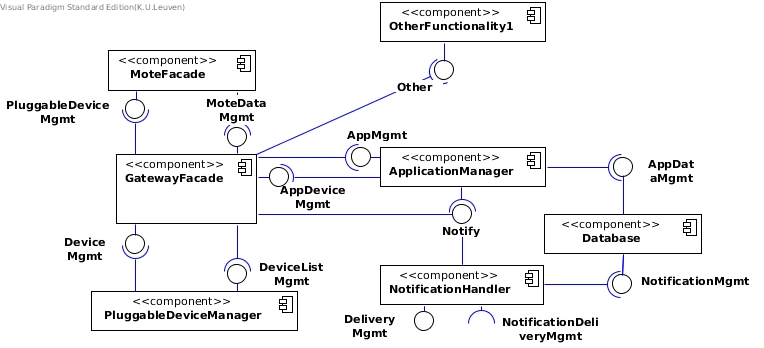
\includegraphics[width=1.00\textwidth]{component-diagram-1}
        	\caption{Component-and-connector diagram of this decomposition.}
            \label{fig:it1-cc_main}
        \end{figure}

        \noindent The responsibilities of the components are as follows:

    \subparagraph{ApplicationManager}
        Responsible for deactivating applications and after this action calls method of
        \texttt{the NotificationHandler} to send notification to a customer organisation.
        When \texttt{the ApplicationManager} detects that application uses failed pluggable devices,
        then the notification is sent to an application.

        set redundancy in the available pluggable devices??
        (Av3) ???? check mandatory user roles

    \subparagraph{Database}
        General database for other data. For instance the Database storages the data
        of notifications (Av3).

    \subparagraph{GatewayFacade}
        Receives heartbeats from pluggable devices and sends heartbeats/device lists.
        \texttt{The GatewayFacade} sends commands to \texttt{the ApplicationManager}
        to shutdown applications, if is it needed. \\

        send notification trigger ???(Av3)\\
        forward data to applications

    \subparagraph{MoteFacade}
        Sends heartbeats from pluggable devices to\texttt{the PluggableDeviceFacade}.

    \subparagraph{NotificationHandler}
        Responsible for send notifications to infrastructure owner, customer organisation
        and applications (Av3). \\
        stored by system \(->\) contact DB? \\
        lookup communication channel \\
        users choose delivery method?

    \subparagraph{PluggableDeviceFacade}
        Sends heartbeats to \texttt{the MoteFacade}.

    \subparagraph{PluggableDeviceManager}
        Checks list of devices and see if there are pluggable devices for applications.
        \texttt{the PluggableDeviceManager} contains application preferences (e.g. amount of sensors required) and
        can send command to deactivate application.
        Send information about new/needed hardware is detected to \texttt{the GatewayFacade}, that sends command to
        reactivate application.
        check redundancy in the available pluggable devices??? is not the same like first sentence???

    % \paragraph{Behaviour}
    % A SEQUENCE DIAGRAM WOULD BE USEFUL FOR
    % UC11: shows how the gateway checks if devices are initialised
    % UC14: shows how applications can get deactivated

    \paragraph{Deployment}
        Figure \ref{fig:it1-depl_main} shows the allocation of components
        to physical nodes.

        \begin{figure}[!htp]
        	\centering
        	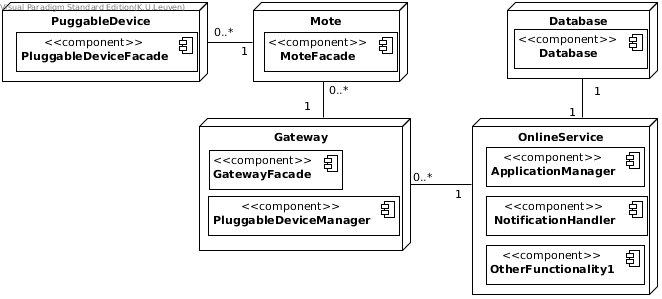
\includegraphics[width=1.00\textwidth]{deployment-diagram-1}
        	\caption{Deployment diagram of this decomposition.}\label{fig:it1-depl_main}
        \end{figure}


\subsection{Interfaces for child modules}\label{add1-interfaces}
    This section describes the interfaces assigned to the components defined
    in the section above. Per interface, we list its methods by means of its
    syntax. The data types used in these interfaces are defined in the following section. \\

    \noindent Each method shows which (part of a) quality attribute or use case caused
    a need for the method. However, this does not mean that a method is
    only to be used to satisfy that quality  attribute or use case, it could
    be used for other causes not yet mentioned here.

    \subsubsection{ApplicationManager}
        \begin{itemize}
            \item ForwardData
            \begin{itemize}
                \item \texttt{void sendData(PluggableDeviceData data)}
                \begin{itemize}
                    \item Effect: Send pluggable device data to an application that wants to use it
                    \item Created for:
                \end{itemize}
            \end{itemize}

            \item AppMgmt
            \begin{itemize}
                \item \texttt{void deactivateApplicationInstance(int applicationInstanceID)}
                \begin{itemize}
                    \item Effect: Deactivates a running instance of an application.
                    \item Created for:
                \end{itemize}
                \item \texttt{void activateApplicationInstance(int applicationInstanceID)}
                \begin{itemize}
                    \item Effect: Activates a new instance of an application.
                    \item Created for:
                \end{itemize}
            \end{itemize}
        \end{itemize}

    \subsubsection{Database}
        \begin{itemize}
            \item NotificationMgmt
            \begin{itemize}
                \item \texttt{int storeNotification(NotificationData data)}
                \begin{itemize}
                    \item Effect: Stores a new notification entry in the database. Returns the id of the new notification.
                    \item Created for:
                \end{itemize}
                \item \texttt{void updateNotification(NotificationData data)}
                \begin{itemize}
                    \item Effect: Updates an existing notification (e.g. change status to "sent").
                    \item Created for:
                \end{itemize}
                \item \texttt{int lookupNotificationChannelForUser(int userID)}
                \begin{itemize}
                    \item Effect: Returns the type of communication channel a user prefers.
                                  Different communication channels are mapped to integers.
                    \item Created for:
                \end{itemize}
            \end{itemize}

            \item AppDataMgmt
            \begin{itemize}
                \item \texttt{void updateApplication(ApplicationData data)}
                \begin{itemize}
                    \item Effect: Updates an application in the database (e.g. change state to 'inactive').
                    \item Created for:
                \end{itemize}
                \item \texttt{void updateSubscription(SubscriptionData data)}
                \begin{itemize}
                    \item Effect: Updates a subscription in the database (e.g. change state to 'disabled').
                    \item Created for:
                \end{itemize}
            \end{itemize}
        \end{itemize}

    \subsubsection{GatewayFacade}
        \begin{itemize}
            \item MoteDataMgmt
            \begin{itemize}
                \item \texttt{void sendHeartbeat(int moteID, List<PluggableDeviceInfo> devices)}
                \begin{itemize}
                    \item Effect: Sends a heartbeat to a certain gateway with information about operational devices.
                    \item Created for:
                \end{itemize}
            \end{itemize}

            \item DeviceMgmt
            \begin{itemize}
                \item \texttt{List<DeviceInfo> getConnectedDevices()}
                \begin{itemize}
                    \item Effect: Describe the effect of calling this operation.
                    \item Created for:
                \end{itemize}
                \item \texttt{void timerExpired(int deviceID)}
                \begin{itemize}
                    \item Effect: Lets the gateway know that a timer for pluggable device or mote has expired.
                                  This will generate a notification for an infrastructure owner.
                    \item Created for:
                \end{itemize}
                \item \texttt{void deactivateApplicationInstance(int applicationInstanceID)}
                \begin{itemize}
                    \item Effect: Deactivates a certain application. This could happen when
                                  mandatory pluggable devices for the application are missing.
                    \item Created for:
                \end{itemize}
                \item \texttt{void reactivateApplicationInstance(int applicationInstanceID)}
                \begin{itemize}
                    \item Effect: Reactivate an application instance. This could happen
                                  automatically after a broken sensor has been replaced.
                    \item Created for:
                \end{itemize}
            \end{itemize}

            \item AppDeviceMgmt
            \begin{itemize}
                \item \texttt{bool areEssentialDevicesOperational(int applicationID)}
                \begin{itemize}
                    \item Effect: Returns true if all essential devices for the application
                                  with id "applicationID" are operational.
                    \item Created for:
                \end{itemize}
            \end{itemize}
        \end{itemize}

    \subsubsection{MoteFacade}
        \begin{itemize}
            \item PluggableDeviceDataMgmt
            \begin{itemize}
                \item \texttt{List<DeviceInfo> getConnectedDevices()}
                \begin{itemize}
                    \item Effect: Returns a list of information about devices that are connected to the mote.
                    \item Created for:
                \end{itemize}
            \end{itemize}
        \end{itemize}

    \subsubsection{NotificationHandler}
        \begin{itemize}
            \item Notify
            \begin{itemize}
                \item \texttt{void notify(int userID, String message)}
                \begin{itemize}
                    \item Effect: Describe the effect of calling this operation.
                    \item Created for:
                \end{itemize}
            \end{itemize}

            \item DeliveryMgmt
            \begin{itemize}
                \item \texttt{void sendAcknowledgement(int notificationID)}
                \begin{itemize}
                    \item Effect: Sends an acknowledgement to the system for a certain notification.
                    \item Created for:
                \end{itemize}
            \end{itemize}
        \end{itemize}

    \subsubsection{External notification delivery serivce}
        \begin{itemize}
            \item NotificationDeliveryMgmt
            \begin{itemize}
                \item \texttt{void notify(JSONObject data)}
                \begin{itemize}
                    \item Effect: Deliver a notification to an end user using a specific delivery service.
                    \item Created for:
                \end{itemize}
            \end{itemize}
        \end{itemize}

    \subsubsection{PluggableDeviceManager}
        \begin{itemize}
        	\item DeviceListMgmt
        	\begin{itemize}
        		\item \texttt{void sendHeartbeat(int moteID, List<PluggableDeviceInfo> devices)}
        		\begin{itemize}
        			\item Effect: Send a heartbeat from a mote to check/update timers for operational devices.
        			\item Created for:
        		\end{itemize}
        		\item \texttt{bool areEssentialDevicesOperational(int applicationID)}
        		\begin{itemize}
        			\item Effect: Returns true if all essential devices for the application
                                  with id "applicationID" are operational.
        			\item Created for:
        		\end{itemize}
        	\end{itemize}
        \end{itemize}


\subsection{Data type definitions}
    This section defines the data types used in the interface descriptions above.

    \paragraph{PluggableDeviceData}
              contains data from a pluggable device at a certain point in time
              (value, type, date) (e.g. a sensor reading, an actuator status)
    \paragraph{PluggableDeviceSettings}
              contains settings for a pluggable device (power status,
              data update rate, ...)
    \paragraph{PluggableDeviceInfo}
              contains information about a pluggable device (device id,
              power status, data update rate, ...)
    \paragraph{NotificationData}
              contains data about a notification (message text, recipient,
              communication channel, date, status, source, ...).
    \paragraph{ApplicationData}
              contains data about an application instance (instance id, running status, ...)
    \paragraph{SubscriptionData}
              contains data about a subscription (subscription id, subscription status,
              subscription period, ...).


\subsection{Verify and refine}
    \noindent The selected architectural drivers have been handled completely
    in this decomposition.
    This section describes per component which (parts of) the remaining
    requirements it is responsible for. If requirements are split in
    multiple parts, this is indicated by the addition of a letter
    (or number, depending on the structure of the requirement) after their title.

    \paragraph{ApplicationManager}
        \begin{itemize}
            \item \emph{Av2}: Application failure \\
                   Prevention: a, b \\
                   Detection: a, b, c \\
                   Resolution: a, b, c
           \item \emph{P1}: Large number of users: c
           \item \emph{M1}: Integrate new sensor or actuator manufacturer: 1.c, 2.a
           \item \emph{M2}: Big data analytics on pluggable data and/or application usage data: d, e
           \item \emph{U1}: Application updates: a, b, c, d
           \item \emph{U2}: Easy Installation: e
           \item \emph{UC12}: Perform actuation command
           \item \emph{UC17}: Activate an application: 3, 4
        \end{itemize}

    \paragraph{Database}
        \begin{itemize}
          	\item None
        \end{itemize}

    \paragraph{GatewayFacade}
        \begin{itemize}
            \item \emph{Av1}: Communication between SIoTIP gateway and Online Service \\
                               Resolution: b, c, d
            \item \emph{M1}: Integrate new sensor or actuator manufacturer: 1.a, 2.b
            \item \emph{U2}: Easy Installation: a, c, d
            \item \emph{UC11}: Send pluggable device data: 1
        \end{itemize}

    \paragraph{MoteFacade}
        \begin{itemize}
            \item \emph{M1}: Integrate new sensor or actuator manufacturer: 1.a, 2.b
            \item \emph{U2}: Easy Installation: b, c, d
            \item \emph{UC04}: Install mote: 1, 2
            \item \emph{UC05}: Uninstall mote: 1
            \item \emph{UC06}: Insert a pluggable device into a mote: 2
            \item \emph{UC07}: Remove a pluggable device from its mote: 2
            \item \emph{UC11}: Send pluggable device data: 1
        \end{itemize}

    \paragraph{NotificationHandler}
        \begin{itemize}
            \item \emph{UC16}: Consult notification message: 5
            \item \emph{UC17}: Activate an application: 5, 6
        \end{itemize}

    \paragraph{OtherFunctionality1}
        \begin{itemize}
            \item \emph{Av1}: Communication between SIoTIP gateway and Online Service \\
                               Detection: a, b, c, d
                               Resolution: a
           	\item \emph{P1}: Large number of users: a
            \item \emph{P2}: Requests to the pluggable data database
            \item \emph{M1}: Integrate new sensor or actuator manufacturer: 1.d
            \item \emph{M2}: Big data analytics on pluggable data and/or application usage data: a
            \item \emph{U2}: Easy Installation: e
            \item \emph{UC01}: Register a customer organisation
            \item \emph{UC02}: Register an end-user
            \item \emph{UC03}: Unregister an end user
            \item \emph{UC04}: Install mote: 3
            \item \emph{UC05}: Uninstall mote: 2.b
            \item \emph{UC06}: Insert a pluggable device into a mote: 3: topology part; alternative 3a.1.b
            \item \emph{UC07}: Remove a pluggable device from its mote: 3.b
            \item \emph{UC08}: Initialise a pluggable device: 1, 2, 4
            \item \emph{UC09}: Configure pluggable device access rights
            \item \emph{UC10}: Consult and configure the topology
            \item \emph{UC11}: Send pluggable device data: 3
            \item \emph{UC13}: Configure pluggable device
            \item \emph{UC16}: Consult notification message: 1, 2, 3, 4
            \item \emph{UC17}: Activate an application: 1, 2
            \item \emph{UC19}: Subscribe to application
            \item \emph{UC20}: Unsubscribe from application
            \item \emph{UC21}: Send invoice
            \item \emph{UC22}: Upload an application
            \item \emph{UC23}: Consult application statistics
            \item \emph{UC24}: Consult historical data
            \item \emph{UC25}: Access topology and available devices
            \item \emph{UC26}: Send application command or message to external front-end
            \item \emph{UC27}: Receive application command or message to external front-end
            \item \emph{UC28}: Log in
            \item \emph{UC29}: Log out
        \end{itemize}

    \paragraph{PluggableDeviceFacade}
        \begin{itemize}
        	\item \emph{U2}: Easy Installation: d
        \end{itemize}

    \paragraph{PluggableDeviceManager}
        \begin{itemize}
            \item \emph{U2}: Easy Installation: c, d
            \item \emph{UC04}: Install mote: 4
            \item \emph{UC05}: Uninstall mote: 2
            \item \emph{UC06}: Insert a pluggable device into a mote: 3: uninitialised part; alternative 3a.1 3a.2 3a.4; 4
            \item \emph{UC07}: Remove a pluggable device from its mote: 3.a, 3.c
            \item \emph{UC08}: Initialise a pluggable device: 3
            \item \emph{UC11}: Send pluggable device data: 2, 3a
        \end{itemize}

\newpage
\section{Decomposition 2: OtherFunctionality1 (M1, P2, UC11)}

\subsection{Module to decompose}
    In this run we decompose OtherFunctionality1.


\subsection{Selected architectural drivers}
    The non-functional drivers for this decomposition are:
    \begin{itemize}
    	\item \emph{M1}: Integrate new sensor or actuator manufacturer
        \item \emph{P2}: Requests to the pluggable data database
    \end{itemize}

    \noindent The related functional drivers are:
    \begin{itemize}
        \item \emph{UC11}: Send pluggable device data (P2) \\
              This use case stores pluggable device data in the pluggable device data storage.
              This could be a sensor reading or an actuator status.
    \end{itemize}

    \paragraph{Rationale}
    We chose M1 as it was one of the remaining quality attributes with high priority.
    M1's focus on easily introducing new types of devices to the system is very important
    because of the fast growing market for IoT and development of applications for IoT.
    Thus, we want to handle this quality attribute before U2 (the other remaining
    attribute with high priority), as we presume that customer organisations
    are more interested in using new devices than the effort it takes for
    infrastructure owners to install the devices. \\
    We also chose P2 because it is strongly related to M1; the whole data flow from
    devices to storage/applications needs to exist before modifications can even be made.
    This combination of M1 and P2 would force us to handle processing and
    storage of data while making the involved components as simple as possible to modify.


\subsection{Architectural design}
    This section describes what needs to be done to satisfy the requirements for
    this decomposition and how involved problems/obstacles are solved.
    % Tactics:
    %     Limit event response? reply within response measure deadlines
    %     Prioritize events
    %     Introduce concurrency
    %     Schedule resources

    % Tactics M1:
    %     reduce size of modules: split module

    \paragraph{M1: Handling new types of pluggable devices}
        The new types of sensor or actuator data should be transmitted, processed and stored,
        and should be made available to applications. The infrastructure managers must be able to initialize the new type of pluggable device
        (UC8 : Initialise a pluggable device), configure access rights for these devices (UC9 : Con-
        figure pluggable device access rights), and view detailed information about the new type
        of pluggable device (UC10 : Consult and configure the topology).

        The developers have to make changes to: component1, component2, datatype X.
        The new type of sensor needs to be able to be initialised so that it can send data.
        Thus, the PluggableDeviceFacade code that initialises devices should be updated for
        each new type of sensor. The PluggableDeviceData datatype should be updated to
        represent the new type of data. In this case, the new type will have to be added
        to the database that contains all different types of sensor data.

    \paragraph{M1: Data conversions}
        The pluggable data processing subsystem should be extended with relevant data conver-
        sions, e.g. converting temperature in degrees Fahrenheit to degrees Celsius.
        \texttt{The PluggableDeviceDataConverter} is resposible for converting data
        in system, for instance converting temperature in degrees Fahrenheit
        to degrees Celsius. System has to work with relevant data,
        otherwise problem may arise.

    \paragraph{M1: Usage of new data by applications}
        The available applications can be updated to use any new pluggable devices.
        This is possible through the RequestData interface provided by PluggableDeviceDataScheduler.
        The application manager can get device data from the PluggableDeviceDB and return this
        data to applications in the PluggableDeviceData datatype. This datatype can easily be
        updated for new types of pluggable devices.

    \paragraph{M1: Configuration of new device by infrastructure owners}
        Initialisation: IO triggers the initialise() method which has been
        updated for the new pluggable device -> OK\\
        Configure access rights: has absolutely fucking nothing to do with the
        new sensor type -> OK \\
        Consult and configure topology: same as configure access rights

    \paragraph{P2: Scheduling}
        - In normal mode, the database processes incoming requests in a first-in-first-out order.
        - If the system fails to comply to the deadlines specified below, it goes in overload mode: requests
            are handled in the order that returns the system to normal mode the fastest, taking into
            account:
            ∗ the nature of the requests: storing new pluggable data (UC11 : Send pluggable device
            data) has priority over specific lookup queries (e.g. retrieving most recent measurement
            for a few sensors), which in turn have priority over broad queries (e.g. retrieving all sensor
            data for the last month).
            ∗ the priority of an application: requests from applications marked as critical by their sub-
            scribers are processed before non-critical applications.
        - Also a mechanism should be in place to avoid starvation of any type of request.

        dynamic priority scheduling \\
        tactics: schedule resource, prioritize events, also limit event response?\\
        starvation avoidance

    \paragraph{P2: Pluggable data separation}
        The processing of (large amounts of) requests concerning pluggable data has no impact on
        requests concerning other data, e.g. available applications.

        "pluggable data has no impact on other data"
        two databases

    \subsubsection{Alternatives considered}
        \paragraph{P2: Alternatives for Scheduling}
        In overload mode, a high priority process will run before a low priority process. 
        It can cuase that the low priority process will never be scheduled.
        Our scheduling algorithms will contain code to guarantee that all processes will 
        receive a minimum amount of each important resource (e.g. CPU time) in order to avoid starvation.


\subsection{Instantiation and allocation of functionality}
    This section describes the new components which instantiate our solutions described
    in the section above and how components are deployed on physical nodes. \\
    Unless stated otherwise the responsibilities assigned in the first decomposition are unchanged.

    \paragraph{Decomposition}
        Figure \ref{fig:it2-cc_main} shows the components resulting from the
        decomposition in this run.

        \begin{figure}[!h]
        	\centering
            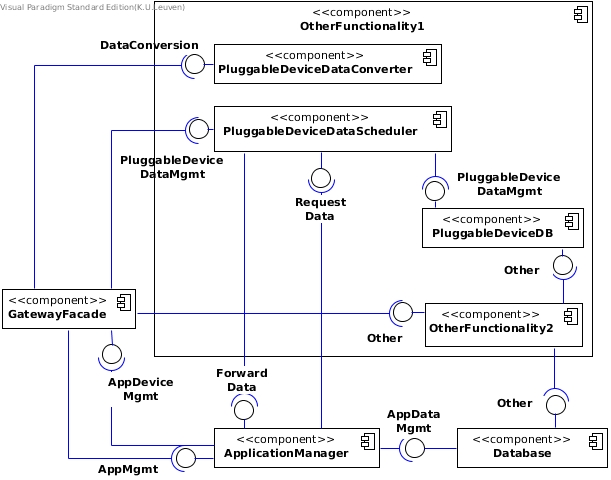
\includegraphics[width=1\textwidth]{component-diagram-2}
        	\caption{Component-and-connector diagram of this decomposition.}
            \label{fig:it2-cc_main}
        \end{figure}

        \noindent The responsibilities of the components are as follows:

    \subparagraph{PluggableDeviceDB}
        stores data related to pluggable devices. In \texttt{the PluggableDeviceDB}
        is stored basic information about devices.

    \subparagraph{PluggableDeviceDataScheduler}
        \texttt{the PluggableDeviceDB} receives a large amount of parallel request
        and it is neccesary to handle with that.
        \texttt{The PluggableDeviceDataScheduler} is resposnsible for scheduling jobs
        that interact with database. Jobs are processed in a first-in-first-out order normaly.
        In case te overload mode is detected, jobs are proccesed in  the  order
        that  returns  the  system. In case the data has to be saved,
        \texttt{The PluggableDeviceDataScheduler} call method for saving the data, that
         \texttt{the PluggableDeviceDB} provides.

    \subparagraph{PluggableDeviceDataConverter}
       is component for conversions of new type of data of new type of device (M1).
       For instance converting temperature is very useful in the system.

    % \paragraph{Behaviour}
        % A SEQUENCE DIAGRAM WOULD BE USEFUL FOR
        % UC11: shows how the gateway checks if devices are initialised
        % UC14: shows how applications can get deactivated

    \paragraph{Deployment}
        Figure \ref{fig:it2-depl_main} shows the allocation of components
        to physical nodes.

        \begin{figure}[!h]
        	\centering
        	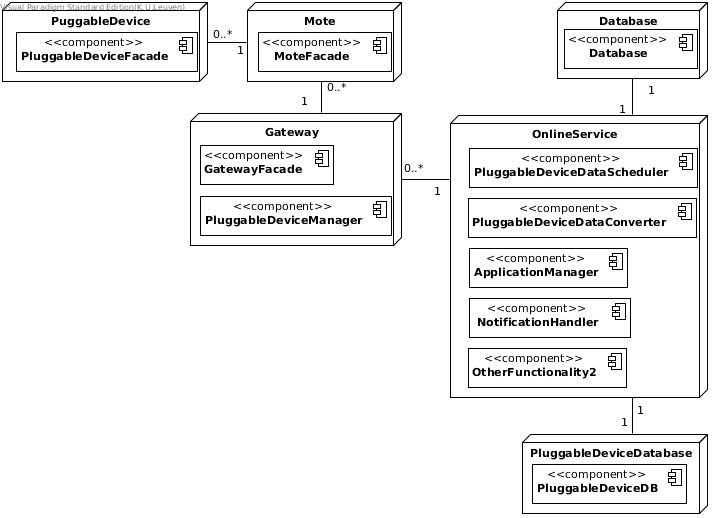
\includegraphics[width=1\textwidth]{deployment-diagram-2}
        	\caption{Deployment diagram of this decomposition.
        	}\label{fig:it2-depl_main}
        \end{figure}


\subsection{Interfaces for child modules}\label{add2-interfaces}
    This section describes the interfaces assigned to the components defined
    in the section above. Per interface, we list its methods by means of its
    syntax. The data types used in these interfaces are defined in the following section. \\

    \noindent Each method shows which (part of a) quality attribute or use case caused
    a need for the method. However, this does not mean that a method is
    only to be used to satisfy that quality  attribute or use case, it could
    be used for other causes not yet mentioned here.

    \noindent The interfaces and methods defined here are to be seen as an
    extension of the interfaces defined in previous sections, unless
    explicitly stated otherwise.

    \subsubsection{GatewayFacade}
        \begin{itemize}
            \item MoteDataMgmt, last defined in section \ref{add1-interfaces}
            \begin{itemize}
                \item \texttt{void sendData(PluggableDeviceData data)}
                \begin{itemize}
                    \item Effect: Sends pluggable device data to the connected mote.
                    \item Created for:
                \end{itemize}
            \end{itemize}

            \item DeviceMgmt, last defined in section \ref{add1-interfaces}
            \begin{itemize}
                \item \texttt{void initialiseDevice(int deviceID, PluggableDeviceSettings settings)}
                \begin{itemize}
                    \item Effect: Initialises a pluggable device for use with the system.
                    \item Created for:
                \end{itemize}
            \end{itemize}

            \item AppDeviceMgmt, last defined in section \ref{add1-interfaces}
            \begin{itemize}
                \item \texttt{void configurePluggableDevice(int deviceID, PluggableDeviceSettings settings)}
                \begin{itemize}
                    \item For: Use case 11 step 3.b
                    \item Effect: Causes certain settings to be set on a pluggable
                          device that the gateway is connected to.
                    \item Created for:
                \end{itemize}
            \end{itemize}
        \end{itemize}

    \subsubsection{MoteFacade}
        \begin{itemize}
            \item PluggableDeviceDataMgmt, last defined in section \ref{add1-interfaces}
            \begin{itemize}
                \item \texttt{void sendData(PluggableDeviceData data)}
                \begin{itemize}
                    \item Effect: Sends pluggable device data to the connected mote.
                    \item Created for:
                \end{itemize}
            \end{itemize}

            \item PluggableDeviceMgmt
            \begin{itemize}
                \item \texttt{void initialise(int deviceID, PluggableDeviceSettings settings)}
                \begin{itemize}
                    \item Effect: Initialises a connected pluggable device according to some settings
                    \item Created for:
                \end{itemize}
            \end{itemize}
        \end{itemize}

    \subsubsection{PluggableDeviceFacade}
        \begin{itemize}
        	\item PluggableDeviceMgmt
        	\begin{itemize}
                \item \texttt{void initialise(PluggableDeviceSettings settings)}
                \begin{itemize}
                    \item Effect: Initialises the pluggable device according to some settings
                    \item Created for:
                \end{itemize}
        	\end{itemize}
        \end{itemize}

    \subsubsection{PluggableDeviceManager}
        \begin{itemize}
        	\item DeviceListMgmt, last defined in section \ref{add1-interfaces}
        	\begin{itemize}
        		\item \texttt{bool isDeviceInitialised(int deviceID)}
        		\begin{itemize}
        			\item Effect: Returns true if the device with id "deviceID" has been initialized.
        			\item Created for:
        		\end{itemize}
        	\end{itemize}
        \end{itemize}

    \subsubsection{PluggableDeviceDataScheduler}
        \begin{itemize}
            \item RequestData
            \begin{itemize}
                \item \texttt{List<PluggableDeviceData> requestData(int applicationID, int deviceID, DateTime from, DateTime to)}
                \begin{itemize}
                    \item Effect: Request data from a specific device in a certain time period
                    \item Created for:
                \end{itemize}
            \end{itemize}

            \item PluggableDeviceDataMgmt
            \begin{itemize}
                \item \texttt{void sendData(PluggableDeviceData data)}
                \begin{itemize}
                    \item Effect: Sends pluggable device data to the scheduler to be processed.
                    \item Created for:
                \end{itemize}
            \end{itemize}
        \end{itemize}

    \subsubsection{PluggableDeviceDB}
        \begin{itemize}
            \item PluggableDeviceDataMgmt
            \begin{itemize}
                \item \texttt{void sendData(PluggableDeviceData data)}
                \begin{itemize}
                    \item Effect: Sends pluggable device data to the DB to be stored.
                    \item Created for:
                \end{itemize}
                \item \texttt{List<PluggableDeviceData> getData(int deviceID, DateTime from, DateTime to)}
                \begin{itemize}
                    \item Effect: Returns data from a specific device in a certain time period.
                    \item Created for:
                \end{itemize}
                \item \texttt{List<int> getApplicationsForDevice(int deviceID)}
                \begin{itemize}
                    \item Effect: Returns a list of applications that can use the device with id "deviceID."
                    \item Created for:
                \end{itemize}
            \end{itemize}
        \end{itemize}


\subsection{Data type definitions}
    This section defines new data types that are used in the interface descriptions above.

    \paragraph{DateTime} Represents an instant in time, typically expressed as a date and time of day.


\subsection{Verify and refine}
    \noindent The selected architectural drivers have been handled completely
    in this decomposition.
    This section describes per component which (parts of) the remaining
    requirements it is responsible for. If requirements are split in
    multiple parts, this is indicated by the addition of a letter
    (or number, depending on the structure of the requirement) after their title.

    \paragraph{ApplicationManager}
        \begin{itemize}
            \item \emph{Av2}: Application failure \\
                   Prevention: a, b \\
                   Detection: a, b, c \\
                   Resolution: a, b, c
           \item \emph{P1}: Large number of users: c
           \item \emph{M2}: Big data analytics on pluggable data and/or application usage data: d, e
           \item \emph{U1}: Application updates: a, b, c, d
           \item \emph{U2}: Easy Installation: e
           \item \emph{UC12}: Perform actuation command
           \item \emph{UC17}: Activate an application: 3, 4
        \end{itemize}

    \paragraph{Database}
        \begin{itemize}
          	\item None
        \end{itemize}

    \paragraph{GatewayFacade}
        \begin{itemize}
            \item \emph{Av1}: Communication between SIoTIP gateway and Online Service \\
                               Resolution: b, c, d
            \item \emph{U2}: Easy Installation: a, c, d
        \end{itemize}

    \paragraph{MoteFacade}
        \begin{itemize}
            \item \emph{U2}: Easy Installation: b, c, d
            \item \emph{UC04}: Install mote: 1, 2
            \item \emph{UC05}: Uninstall mote: 1
            \item \emph{UC06}: Insert a pluggable device into a mote: 2
            \item \emph{UC07}: Remove a pluggable device from its mote: 2
        \end{itemize}

    \paragraph{NotificationHandler}
        \begin{itemize}
            \item \emph{UC16}: Consult notification message: 5
            \item \emph{UC17}: Activate an application: 5, 6
        \end{itemize}

    \paragraph{OtherFunctionality2}
        \begin{itemize}
            \item \emph{Av1}: Communication between SIoTIP gateway and Online Service \\
                               Detection: a, b, c, d
                               Resolution: a
           	\item \emph{P1}: Large number of users: a
            \item \emph{M2}: Big data analytics on pluggable data and/or application usage data: a
            \item \emph{U2}: Easy Installation: e
            \item \emph{UC01}: Register a customer organisation
            \item \emph{UC02}: Register an end-user
            \item \emph{UC03}: Unregister an end user
            \item \emph{UC04}: Install mote: 3
            \item \emph{UC05}: Uninstall mote: 2.b
            \item \emph{UC06}: Insert a pluggable device into a mote: 3: topology part; alternative 3a.1.b
            \item \emph{UC07}: Remove a pluggable device from its mote: 3.b
            \item \emph{UC08}: Initialise a pluggable device: 1, 2, 4
            \item \emph{UC09}: Configure pluggable device access rights
            \item \emph{UC10}: Consult and configure the topology
            \item \emph{UC13}: Configure pluggable device
            \item \emph{UC16}: Consult notification message: 1, 2, 3, 4
            \item \emph{UC17}: Activate an application: 1, 2
            \item \emph{UC19}: Subscribe to application
            \item \emph{UC20}: Unsubscribe from application
            \item \emph{UC21}: Send invoice
            \item \emph{UC22}: Upload an application
            \item \emph{UC23}: Consult application statistics
            \item \emph{UC24}: Consult historical data
            \item \emph{UC25}: Access topology and available devices
            \item \emph{UC26}: Send application command or message to external front-end
            \item \emph{UC27}: Receive application command or message to external front-end
            \item \emph{UC28}: Log in
            \item \emph{UC29}: Log out
        \end{itemize}

    \paragraph{PluggableDeviceDB}
        \begin{itemize}
            \item \emph{M2}: Big data analytics on pluggable data and/or application usage data: b
        \end{itemize}

    \paragraph{PluggableDeviceFacade}
        \begin{itemize}
        	\item \emph{U2}: Easy Installation: d
        \end{itemize}

    \paragraph{PluggableDeviceManager}
        \begin{itemize}
            \item \emph{U2}: Easy Installation: c, d
            \item \emph{UC04}: Install mote: 4
            \item \emph{UC05}: Uninstall mote: 2
            \item \emph{UC06}: Insert a pluggable device into a mote: 3: uninitialised part; alternative 3a.1 3a.2 3a.4; 4
            \item \emph{UC07}: Remove a pluggable device from its mote: 3.a, 3.c
            \item \emph{UC08}: Initialise a pluggable device: 3,
        \end{itemize}

    \paragraph{PluggableDeviceDataScheduler}
        \begin{itemize}
            \item \emph{P1}: Large number of users: b
            \item \emph{M2}: Big data analytics on pluggable data and/or application usage data: b, c
        \end{itemize}


\chapter{Resulting partial architecture}\label{sec:architecture}
\sout{This section provides an overview of the architecture constructed through ADD.}\\
\textit{"Since you are a two-student team, you can skip the final step of the
assignment/report ("2. Resulting architecture This section should present
the component diagram of the overall system (after two decompositions).
At this point, you are not required to provide the deployment diagram
of the overall system.")"}

\noindent Figure \ref{comp-whole} shows the whole deployment diagram after
second decomposition.

\begin{sidewaysfigure}[htp]
    \centering
    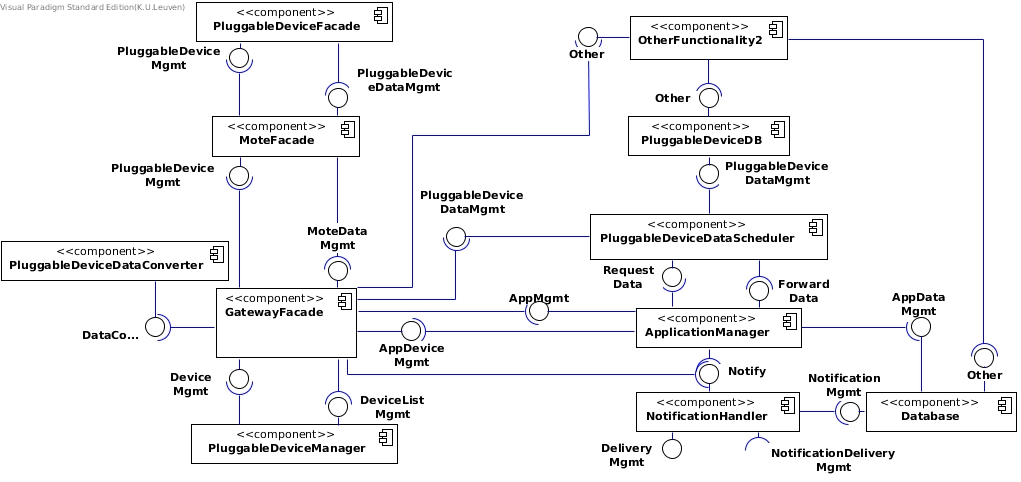
\includegraphics[width=1.00\textwidth]{component-diagram-whole}
    \caption{Complete deployment diagram after second decomposition.}\label{comp-whole}
\end{sidewaysfigure}

\end{document}
